\section{Experiment Definition}
\subsection{Research Goal}
Following the GQM framework proposed by Wohlin et al. \cite{wohlin2012experimentation}, the goal of this research is to \emph{analyze} music streaming applications \emph{for the purpose of} evaluation \emph{with respect to} energy consumption \emph{from the point of view of} users \emph{in the context of} Android applications. Figure 1 presents the visual representation of GQM. 
\begin{figure}[htbp]
 \centering
 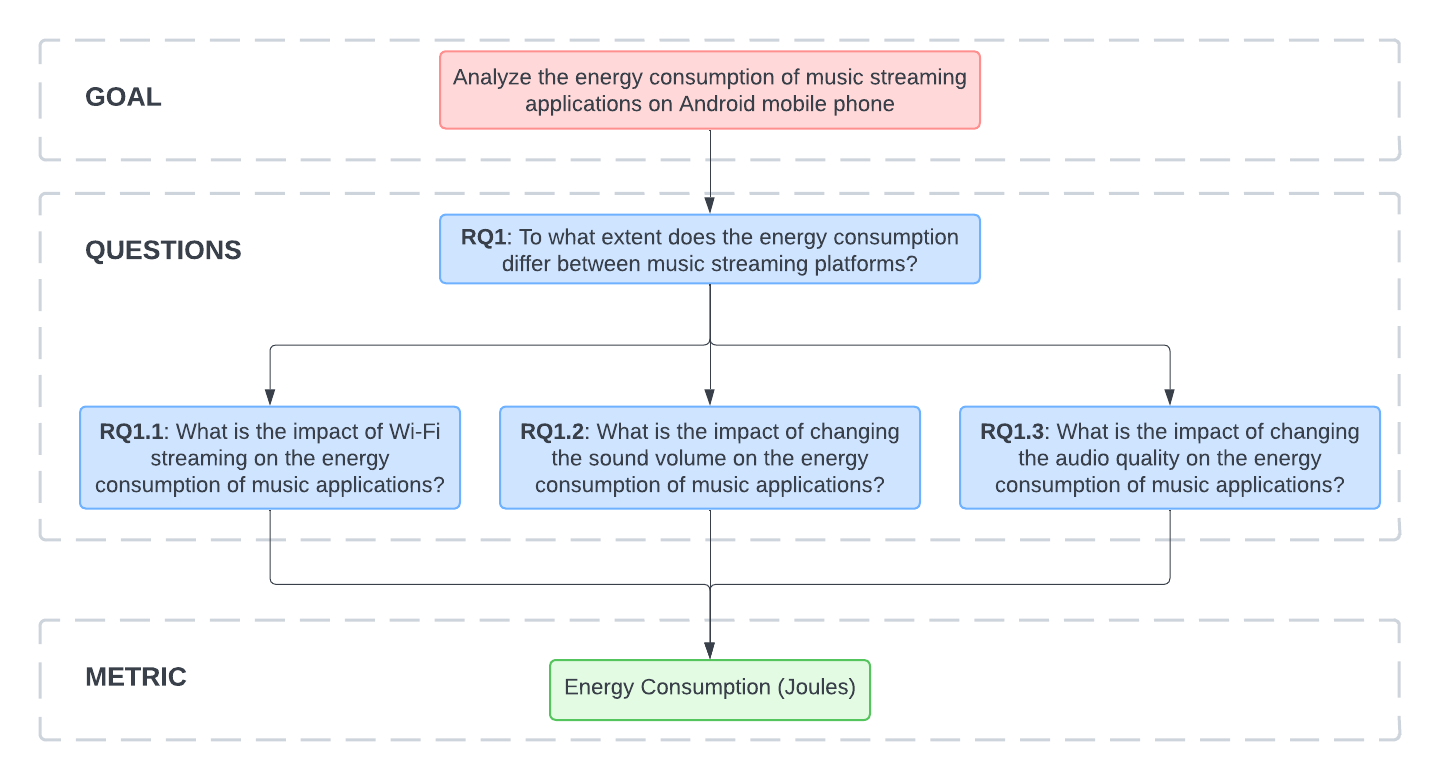
\includegraphics[width=0.8\linewidth]{figures/Visual representation of GQM.png}\textcolor{blue}{\caption{{\color{blue}Visual representation of GQM}}}
\end{figure}
\subsection{Research Questions}
To achieve the aforementioned goal, this study aims at answering one major research question (RQ1) and a set of subquestions (RQ1.1 - 1.3).

\textbf{[RQ 1]}: \emph{To what extent does the energy consumption differ between music streaming platforms?}

In general, users will be challenged by choosing from massive music players. It is not trivial for them to take energy efficiency into consideration as the battery drainage issue poses a negative impact on user experience. This question is intended to inform Android mobile devices users of the energy consumption of different music applications so that they can make a conscious decision to satisfy their requirements. 

To address this question, we compute the energy consumption of Spotify and YouTube Music based on their global popularity. According to Statista, Spotify and YouTube Music are two of the most popular music applications that recorded 13.37M and 9.42M downloads from Android users in June, 2022 \cite{13}. We subscribe to both premium versions to unlock the “very high” audio quality for later use. In order to assure the data integrity and validity, the energy consumption is measured based on a specific duration via internal speakers. Different settings are implemented as they might affect the energy consumption. We identify three possible factors that may cause sharp battery drop. They are:

1. Wi-Fi streaming vs. downloaded playing

\textcolor{blue}{2. Sound volume (\ie low, medium, and high)}

3. Audio quality (\ie , low, normal, high, and very high)

Plus,  They are formulated as sub-questions depicted below.  

  

\textbf{[RQ 1.1]}: \emph{What is the impact of Wi-Fi streaming on the energy consumption of music applications?}

In terms of saving the battery, a broad consensus is that users should avoid streaming as much as possible and play the downloaded music instead. During Wi-Fi streaming, data is exchanged over the Internet, and hence, more battery usage. It is noteworthy that both Spotify and YouTube Music store recently played songs in the cache automatically to provide buffering in case of the sudden connection error. Strictly speaking, users will not keep streaming over the same song even if it has not been downloaded yet. That is to say, Wi-Fi streaming only works the first time the user plays the song. In order to rule out the potential impact that cache might have, we compare the energy consumption caused by Wi-Fi streaming with cache cleared and downloaded file playing. 


{\color{blue}\textbf{[RQ 1.2]}: \emph{What is the impact of changing the sound volume on the energy consumption of music applications?}

Volume is decided by the amplitude of a wave, which further depends on how much energy is transferred. A speaker converts electrical energy to mechanical energy to move air to produce sound waves. The louder the sound, the more electrical energy to put in. Android devices usually have sixteen volume levels ranging from 0 (\ie mute) to 15. We select level 1, level 8, and level 15 as low, medium, and high.}

\textbf{[RQ 1.3]}: \emph{What is the impact of changing the audio quality on the energy consumption of music applications?}

 It is noticeable that the energy consumption varies based on the audio quality because the higher the quality the more data it will use up. Accordingly, frequent data transmission leads to more battery usage. {\color{blue}Both applications provide four kinds of audio quality: low, normal, high, and very high for Spotify whereas low, normal, high, always high for YouTube Music. The default audio quality settings of both applications are normal. It is worth mentioning that we rule out the “high” option in YouTube Music because in this setting, the application will adjust the audio quality automatically based on Internet condition.} We switch between all options to measure the energy consumption respectively. 
 
To ensure that experiment results can be interrupted correctly and consistently, one metric Energy Consumption, measured in Joule (J), is introduced to represent the total energy consumed over the duration. 



% Report about the GQM (with figure).

% \textcolor{red}{Page limit: 2}


